\chapter{Project Design}

This chapter details the design and implementation of the models and algorithms used in this study. The goal is to simulate the spread of infectious diseases on different network structures and apply source detection algorithms to identify the origins of the infection. The design choices, methodologies, and tools used in this study are discussed comprehensively.

\section{Model Structures and Algorithm Implementation}

In our study, we implemented both grid-based and complex network models to explore the dynamics of infectious disease spread. The grid-based models offer simplicity and structured analysis, while the complex network models provide a more realistic representation of real-world interactions.

\subsection{Grid-based models}

The grid-based model is a fundamental approach in epidemiological studies. It represents the population as nodes in a grid, where each node can be in one of several states: susceptible, infected, or recovered. The disease spreads to neighboring nodes based on defined rules. The structure of the grid-based model is illustrated in Figure \ref{fig:grid_model_structure}.

\begin{figure}[H]
    \centering
    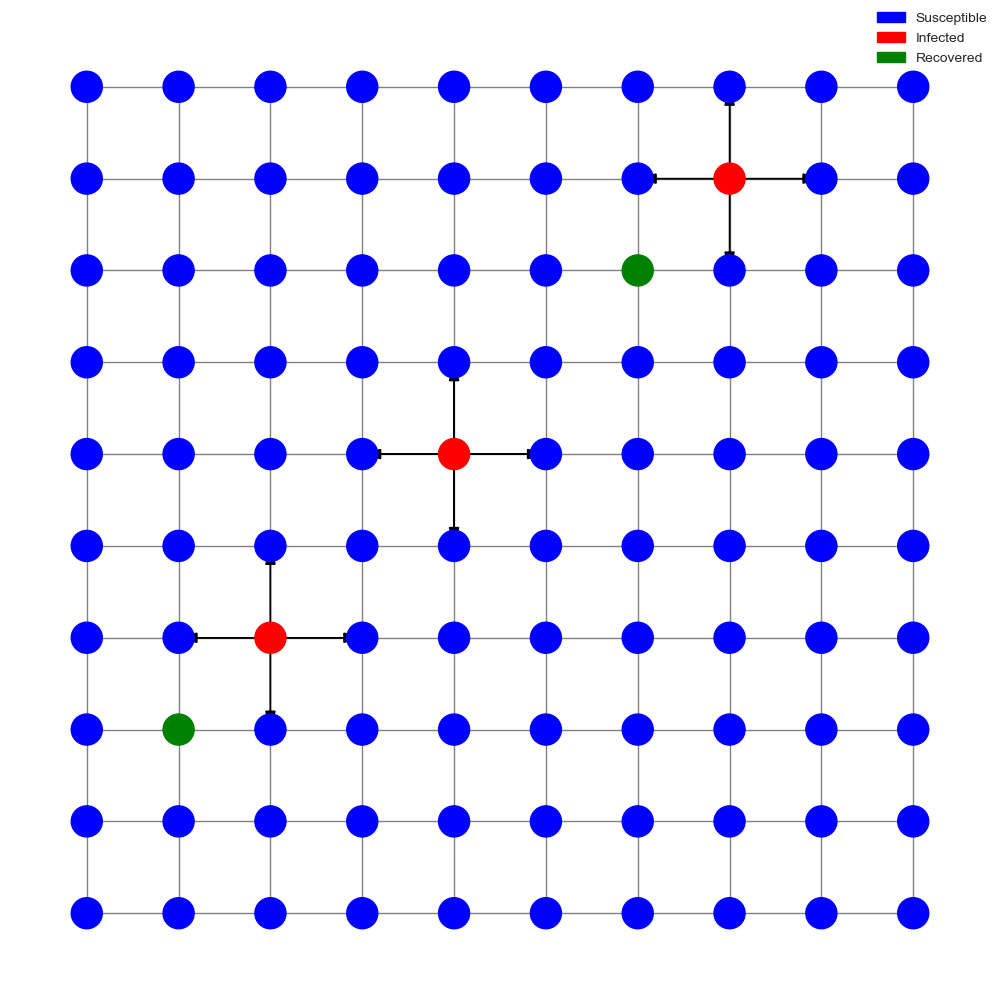
\includegraphics[width=0.6\textwidth]{grid_model_structure.png}
    \caption{Structure of the Grid-Based Model}
    \label{fig:grid_model_structure}
\end{figure}

For source detection within the grid-based model, we implemented three primary algorithms: Jordan Center Identification using Breadth-First Search (BFS), Euclidean Distance Minimization, and Center of Mass Identification. These algorithms were evaluated based on their accuracy, complexity, and ability to handle boundary conditions. The performance comparison of these algorithms is shown in Figure \ref{fig:grid_algorithm_performance}.

\begin{figure}[H]
    \centering
    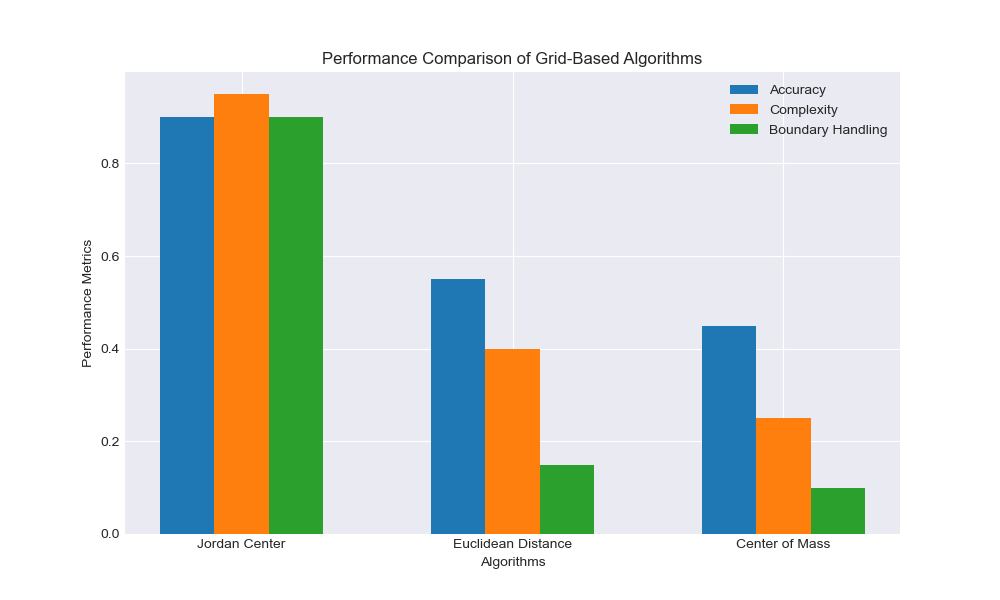
\includegraphics[width=0.8\textwidth]{grid_algorithm_performance.png}
    \caption{Performance Comparison of Grid-Based Algorithms}
    \label{fig:grid_algorithm_performance}
\end{figure}

The \textbf{Jordan Center algorithm} employs a Breadth-First Search (BFS) approach to identify the central node that minimizes the maximum distance to all other nodes. This method calculates the centrality score for each candidate node, selecting the node with the highest score as the source. The detailed implementation of this algorithm is presented in the Implementation chapter.\\

Figures \ref{fig:source_recovery_30_70_fixed_grid}, \ref{fig:source_recovery_30_70_wrap_around_grid}, and \ref{fig:source_recovery_48_51} illustrate the performance of the Jordan Center algorithm in different grid configurations. These images represent the results of running the source location algorithm on 400 different grids at each time step, with each grid being a 100x100 grid.

\begin{figure}[H]
    \centering
    \includegraphics[width=0.8\textwidth]{source_recovery_30_70_Fixed_Grid.png}
    \caption{Source Recovery (30, 70) with a Fixed Grid with Jordan Center Algorithm}
    \label{fig:source_recovery_30_70_fixed_grid}
\end{figure}

Figure \ref{fig:source_recovery_30_70_fixed_grid} shows the performance of the Jordan Center algorithm in a fixed boundary grid. The accuracy of source recovery decreases significantly as the infection reaches the boundaries. This is because edge nodes have fewer neighbors, which skews the centrality calculations, leading to less accurate source detection.

\begin{figure}[H]
    \centering
    \includegraphics[width=0.8\textwidth]{source_recovery_30_70_Wrap_Around_Grid.png}
    \caption{Source Recovery (30, 70) with a Wrap-Around Grid with Jordan Center Algorithm}
    \label{fig:source_recovery_30_70_wrap_around_grid}
\end{figure}

In contrast, Figure \ref{fig:source_recovery_30_70_wrap_around_grid} illustrates the performance of the Jordan Center algorithm in a wrap-around grid configuration. The accuracy remains high due to consistent node behavior across the grid. The wrap-around boundaries eliminate the edge effects seen in fixed boundary grids, allowing for more accurate centrality measurements and, consequently, more precise source detection.

\begin{figure}[H]
    \centering
    \includegraphics[width=0.8\textwidth]{source_recovery_48_51.png}
    \caption{Source Recovery (48, 51) with Jordan Center Algorithm}
    \label{fig:source_recovery_48_51}
\end{figure}

Figure \ref{fig:source_recovery_48_51} demonstrates the high effectiveness of the Jordan Center algorithm when detecting the source at central nodes. The symmetric conditions in the center of the grid favor accurate source detection due to uniform connectivity of nodes.\\

The \textbf{Jordan Center algorithm} performs exceptionally well in wrap-around grid configurations due to the consistent node behavior across the grid. This consistency allows for accurate centrality measurements, resulting in high source recovery accuracy. However, in fixed boundary grids, the algorithm's performance deteriorates as the infection reaches the boundaries. This analysis provides critical insights into selecting and adapting source detection algorithms based on the grid configuration and boundary conditions in epidemiological models.\\

We then explored the \textbf{Center of Mass Algorithm} for source detection. The Center of Mass algorithm calculates the mean position of all infected nodes and designates this point as the source of the infection. While this method is computationally efficient, it has limitations in terms of accuracy, particularly near the boundaries of the grid.

Initially, we applied the Center of Mass algorithm to detect the source node using the regular method. The results are depicted in Figure \ref{fig:source_recovery_48_51_Center_of_Mass}, which shows a poor recovery of the source node. However, upon analyzing the distance of error between the true source node and the recovered one, we observed that the error distance was usually small, especially in the initial stages of the infection spread.

\begin{figure}[H]
    \centering
    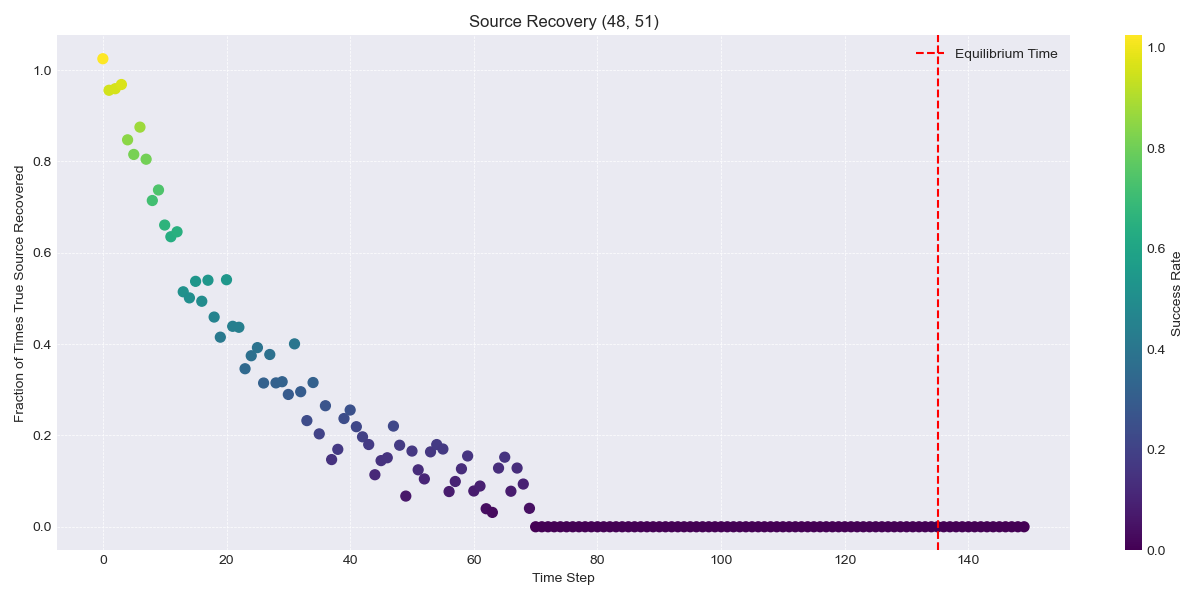
\includegraphics[width=0.8\textwidth]{source_recovery_48_51_Center_of_Mass.png}
    \caption{Source Recovery (48, 51) with Center of Mass Algorithm}
    \label{fig:source_recovery_48_51_Center_of_Mass}
\end{figure}

Given the proximity of the recovered nodes to the true source, we considered an approximation approach, allowing for a \textit{one-node error margin}. This means that if the true source node is a neighbor of the recovered source node, it is considered a successful recovery. When we applied this approximation, the source recovery improved significantly, as shown in Figure \ref{fig:approx_source_recovery_48_51_Center_of_Mass}.

\begin{figure}[H]
    \centering
    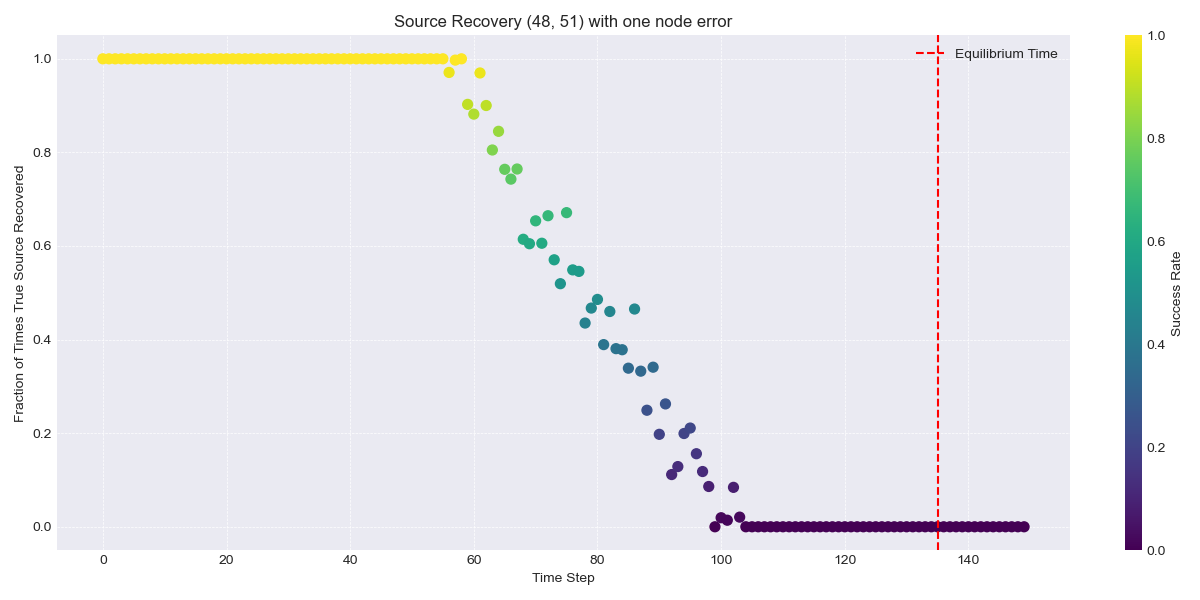
\includegraphics[width=0.8\textwidth]{approx_source_recovery_48_51_Center_of_Mass.png}
    \caption{Approximate Source Recovery (48, 51) with Center of Mass Algorithm allowing one-node error}
    \label{fig:approx_source_recovery_48_51_Center_of_Mass}
\end{figure}

However, the Center of Mass algorithm's performance near the boundaries remained poor, regardless of whether the grid had wrap-around or fixed boundaries. This is illustrated in Figure \ref{fig:approx_source_recovery_30_70_Center_of_Mass}, where the handling of boundary conditions showed poor performance.

\begin{figure}[H]
    \centering
    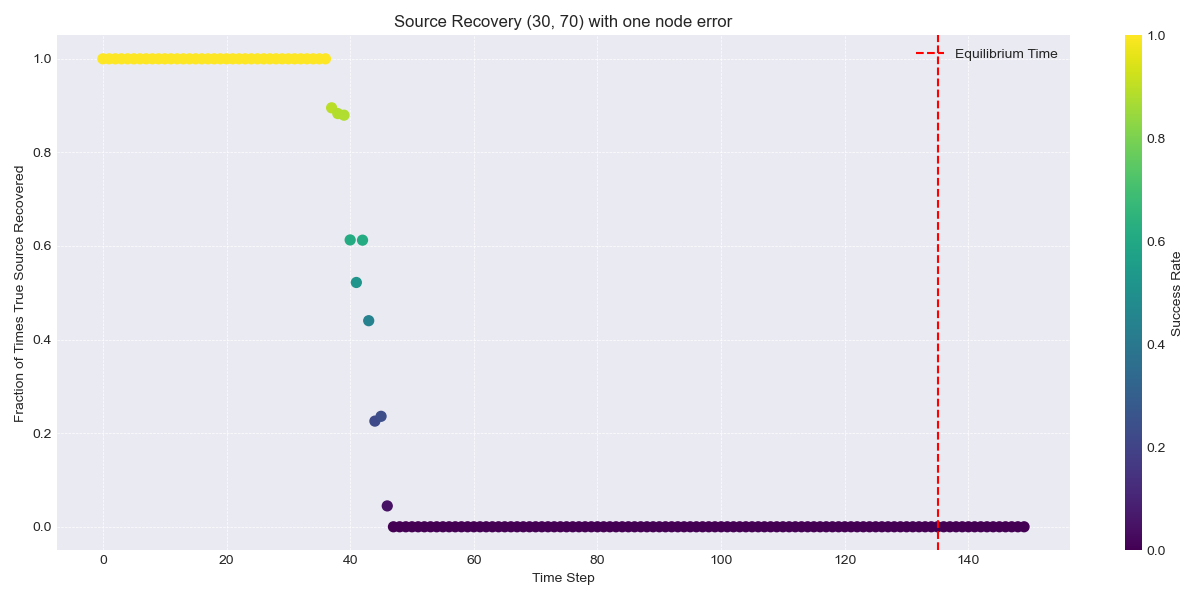
\includegraphics[width=0.8\textwidth]{approx_source_recovery_30_70_Center_of_Mass.png}
    \caption{Approximate Source Recovery (30, 70) with Center of Mass Algorithm allowing one-node error}
    \label{fig:approx_source_recovery_30_70_Center_of_Mass}
\end{figure}

In addition to the source recovery analysis, we analyzed the distance error between the predicted source and the true source over time. This is depicted in Figure \ref{fig:distance_error_true_predicted_source_center_mass}, which shows that the distance error remains relatively small in the initial stages of infection spread, justifying the one-node error margin approximation.

\begin{figure}[H]
    \centering
    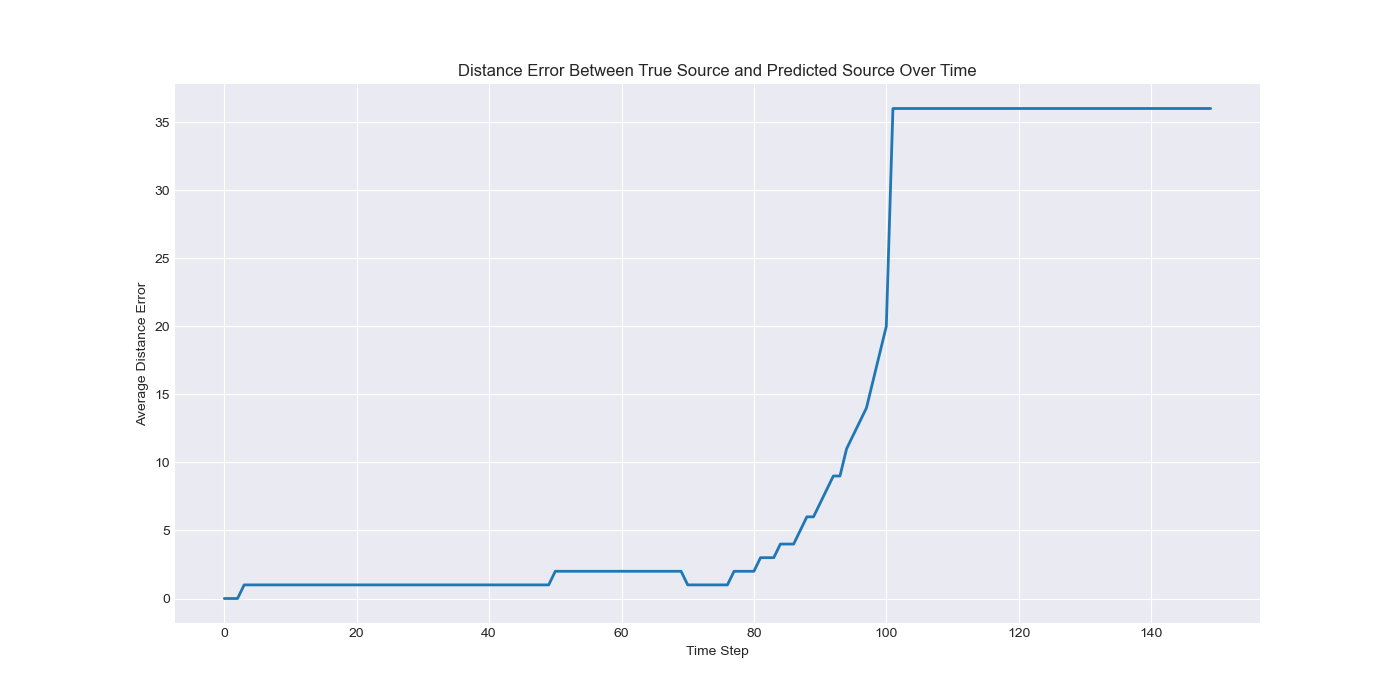
\includegraphics[width=0.8\textwidth]{Distance_Error_True_Predicted_Source_Center_Mass.png}
    \caption{Distance Error Between True Source and Predicted Source Over Time with Center of Mass Algorithm}
    \label{fig:distance_error_true_predicted_source_center_mass}
\end{figure}

Next, we examined the \textbf{Distance Analysis Algorithm}, utilizing Manhattan or Euclidean Distance to identify the source of infection. The algorithm determines the node whose cumulative distance to all infected nodes is minimized. This method, while fast, suffers from inaccuracies near boundaries.

Initially, the Distance Analysis algorithm demonstrated significant errors in identifying the exact source node. However, when we considered the approximate approach, allowing for a \textit{one-node error margin}, the performance improved markedly. Figure \ref{fig:Approx_Source_Recovery_48_51_Distance_Analysis} shows the results for the central node scenario, indicating better recovery rates.

\begin{figure}[H]
    \centering
    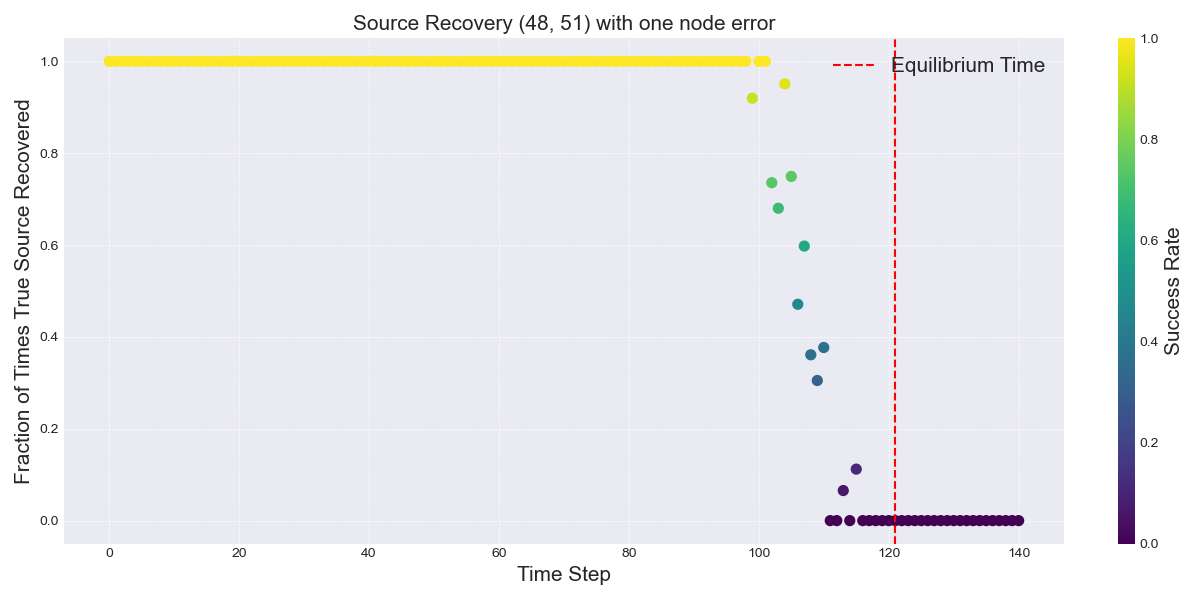
\includegraphics[width=0.8\textwidth]{Approx_Source_Recovery_48_51_Distance_Analysis.png}
    \caption{Approximate Source Recovery (48, 51) with Distance Analysis Algorithm allowing one-node error}
    \label{fig:Approx_Source_Recovery_48_51_Distance_Analysis}
\end{figure}

In boundary conditions, the Distance Analysis algorithm performed poorly, as illustrated in Figure \ref{fig:Approx_Source_Recovery_30_70_Distance_Analysis}. The accuracy significantly drops when the infection reaches the boundaries, indicating a loss of critical information for source detection.

\begin{figure}[H]
    \centering
    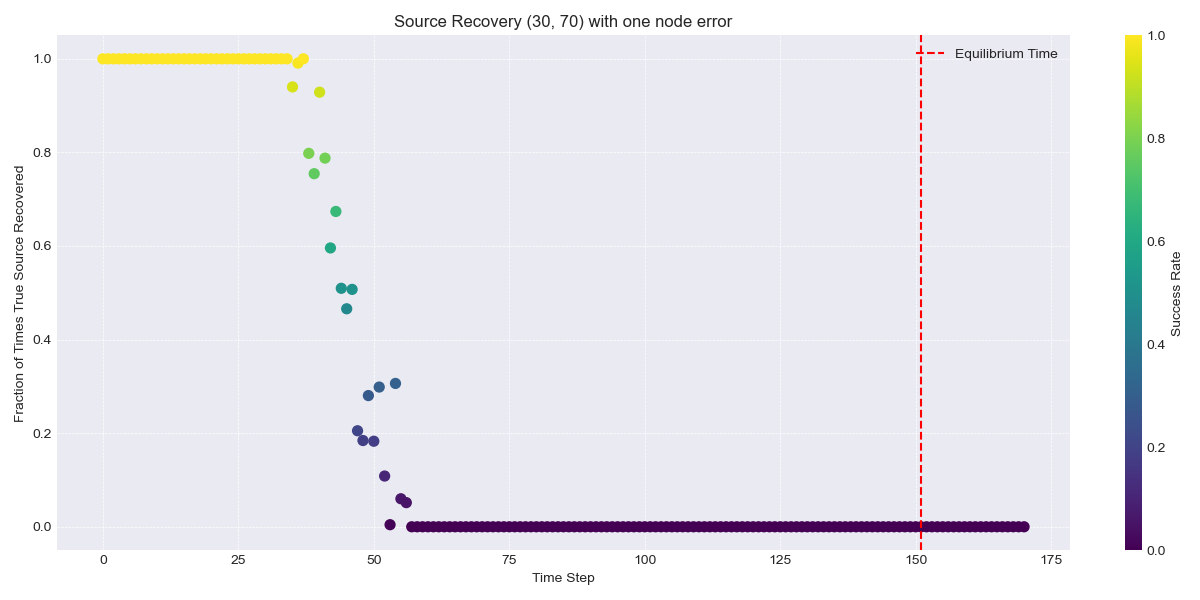
\includegraphics[width=0.8\textwidth]{Approx_Source_Recovery_30_70_Distance_Analysis.png}
    \caption{Approximate Source Recovery (30, 70) with Distance Analysis Algorithm allowing one-node error}
    \label{fig:Approx_Source_Recovery_30_70_Distance_Analysis}
\end{figure}

For a more detailed view, Figure \ref{fig:source_recovery_30_70_Distance_Analysis} shows the performance of the Distance Analysis algorithm without allowing for a one-node error margin, which clearly demonstrates the inadequacy of the approach near the grid boundaries.

\begin{figure}[H]
    \centering
    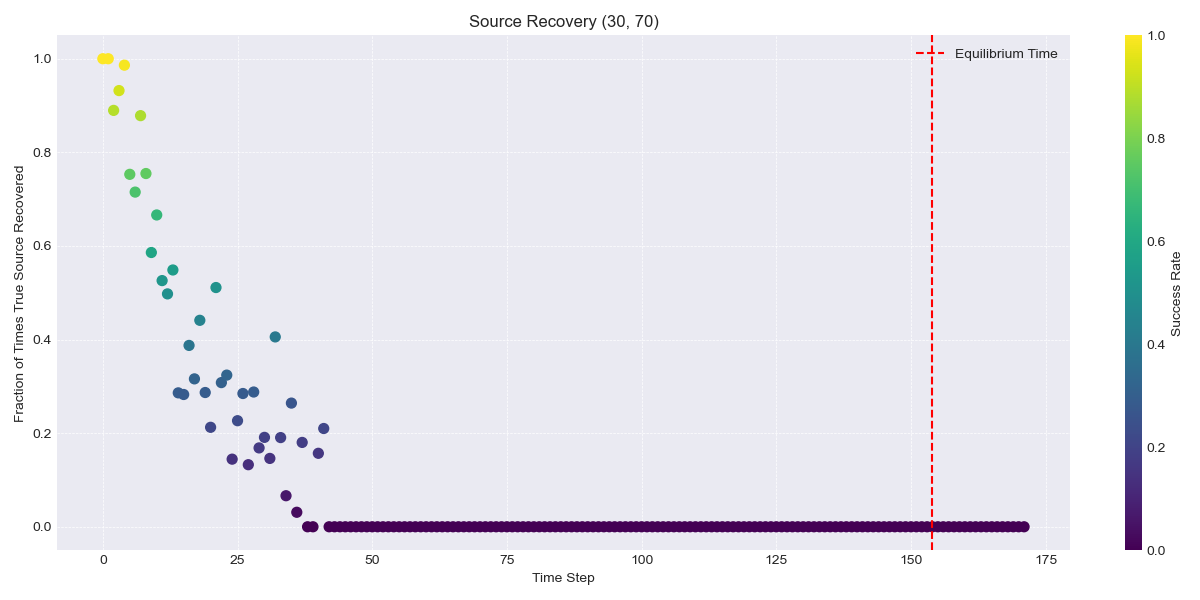
\includegraphics[width=0.8\textwidth]{Source_Recovery_30_70_Distance_Analysis.png}
    \caption{Source Recovery (30, 70) with Distance Analysis Algorithm without one-node error margin}
    \label{fig:source_recovery_30_70_Distance_Analysis}
\end{figure}

Upon comparing the three algorithms, the Jordan Center algorithm consistently demonstrated the highest accuracy in source detection, particularly in wrap-around grid configurations. This can be attributed to its ability to handle uniform connectivity across the grid, which is not affected by boundary conditions. The Center of Mass and the Distance Analysis algorithms, while computationally efficient, showed limitations in accuracy, especially near grid boundaries. The one-node error margin approach significantly improved their performances, making them a viable option for quick approximations.\\

In summary, the grid-based algorithms implemented in this study provided valuable insights into the effectiveness of different approaches for source detection in epidemiological models. The Jordan Center algorithm emerged as the most accurate, especially in wrap-around grid configurations, making it suitable for both grid-based and complex network models. The Center of Mass and Distance Analysis algorithms, while less accurate, offered computational efficiency and improved performance with the one-node error margin approach.\\

Moving forward, we will explore the application of these algorithms to complex network models to further enhance our understanding of disease spread dynamics and improve the traceability of infection sources.

\subsection{Centrality Measures in Complex Network Models}

We move on now to complex network models, which are crucial for a comprehensive understanding of disease spread dynamics in real-world scenarios. Unlike grid-based models, complex networks exhibit diverse structures and connectivity patterns that significantly influence the spread of infections. We used several types of complex networks, including Erdős–Rényi graphs, Random Regular graphs, and Random Geometric graphs. These network types are illustrated in Figure \ref{fig:network_types}.

\begin{figure}[H]
    \centering
    \begin{subfigure}{0.3\textwidth}
        \centering
        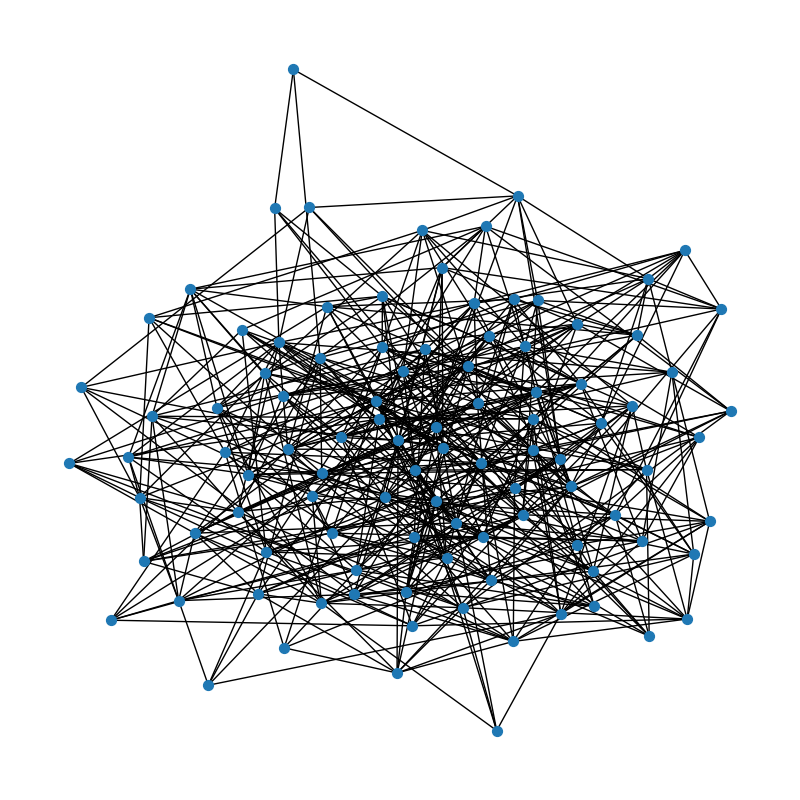
\includegraphics[width=\textwidth]{erdos_renyi_graph.png}
        \caption{Erdős–Rényi Graph}
        \label{fig:erdos_renyi_graph}
    \end{subfigure}
    \begin{subfigure}{0.3\textwidth}
        \centering
        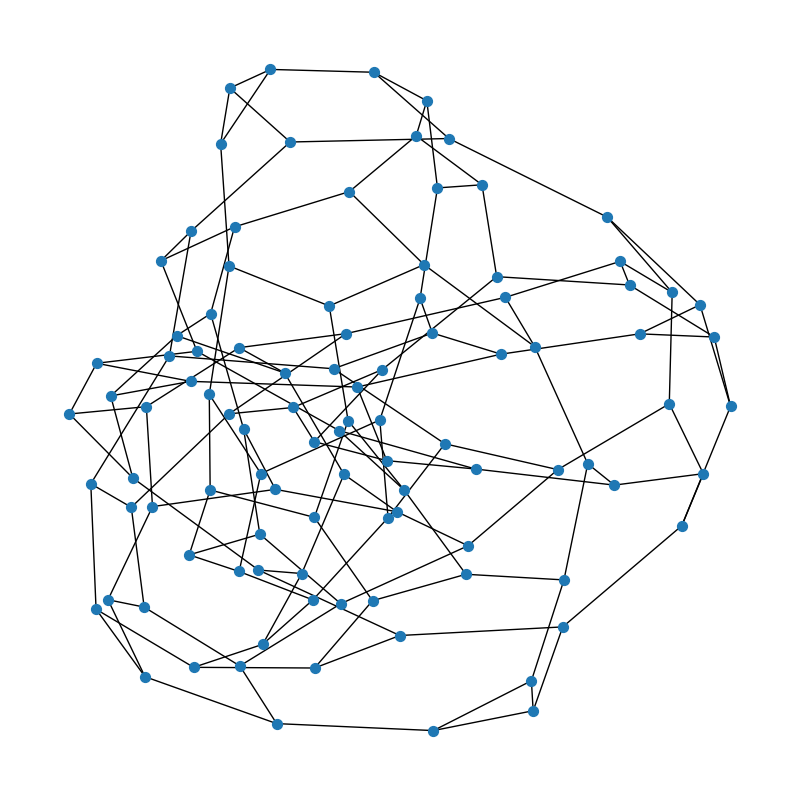
\includegraphics[width=\textwidth]{random_regular_graph.png}
        \caption{Random Regular Graph}
        \label{fig:random_regular_graph}
    \end{subfigure}
    \begin{subfigure}{0.3\textwidth}
        \centering
        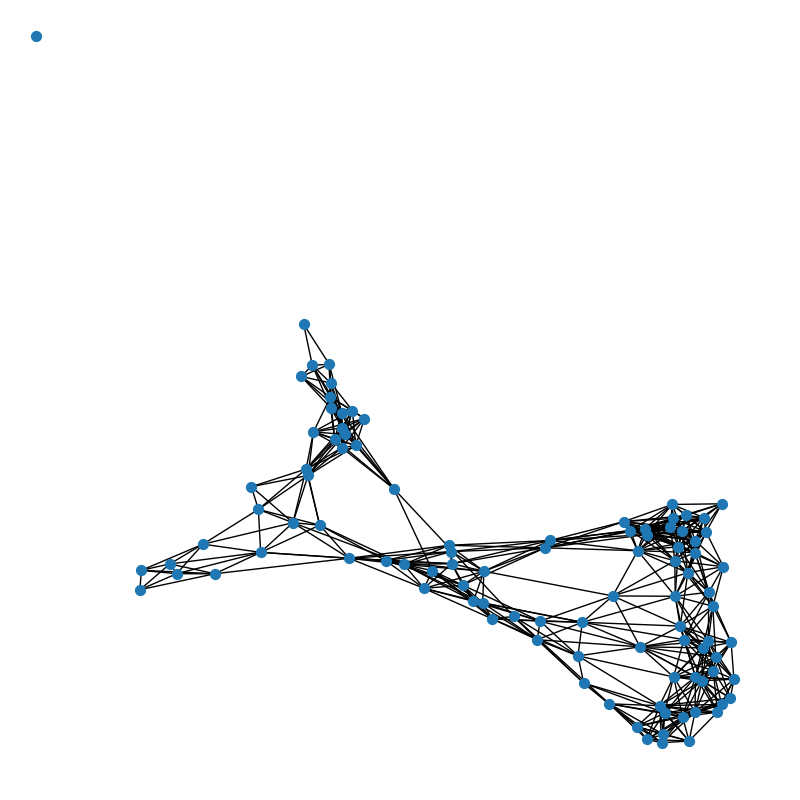
\includegraphics[width=\textwidth]{random_geometric_graph.png}
        \caption{Random Geometric Graph}
        \label{fig:random_geometric_graph}
    \end{subfigure}
    \caption{Examples of Complex Network Structures}
    \label{fig:network_types}
\end{figure}

We chose these networks due to their varying structural properties. Erdős–Rényi graphs are simple random graphs where each edge is included with a fixed probability. Random Regular graphs have a fixed degree for each node, ensuring uniform connectivity. Random Geometric graphs represent spatial networks where nodes are connected if they are within a certain distance, introducing heterogeneity in node degrees.\\

To enhance source detection in these complex networks, we employed various centrality measures \cite{jiang2017}:

\begin{enumerate}
    \item \textbf{Eccentricity + Closeness Centrality:} This combined measure uses both eccentricity and closeness scores to identify central nodes. 
    \item \textbf{Eccentricity:} Defined as the greatest distance between a node and any other node in the network, used to find the "central" node \cite{newman2010}.
    \item \textbf{Betweenness Centrality:} Measures the extent to which a node lies on the shortest paths between other nodes, highlighting nodes critical for the flow of infection \cite{girvan2002}.
    \item \textbf{Eigenvector Centrality:} Assigns relative scores to all nodes based on the principle that connections to high-scoring nodes contribute more to a node's score.
    \item \textbf{Closeness Centrality:} Measures the average length of the shortest path from a node to all other nodes in the network, indicating how quickly information spreads from a given node to others.
\end{enumerate}

The implementation of these centrality measures was integrated into the network simulation, and their performance was tested on various network structures. The evaluation criteria included accuracy and time complexity under varying network conditions and infection parameters.\\

Figure \ref{fig:centrality_measures_explained} from Jiang et al. \cite{jiang2017} provides a comprehensive illustration of these centrality measures.

\begin{figure}[H]
    \centering
    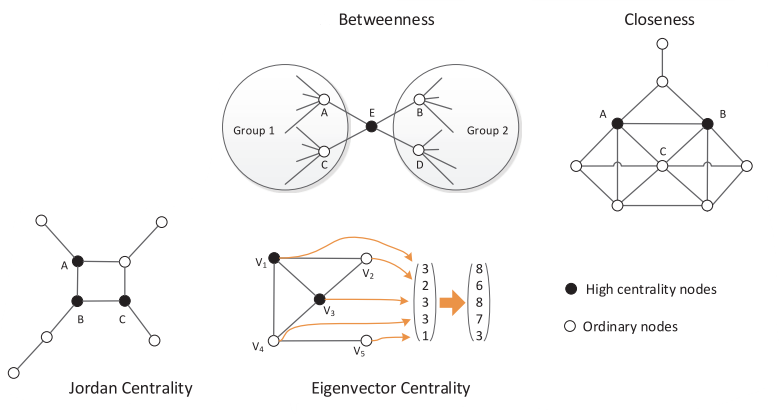
\includegraphics[width=0.8\textwidth]{centrality_measures.png}
    \caption{Centrality Measures Explained (Jiang et al., 2017)}
    \label{fig:centrality_measures_explained}
\end{figure}

In this figure, different centrality measures are visually explained:
\begin{itemize}
    \item \textbf{Betweenness:} Nodes that frequently appear on shortest paths between other nodes.
    \item \textbf{Closeness:} Nodes that can reach other nodes most quickly.
    \item \textbf{Jordan:} Nodes that minimize the maximum distance to other nodes.
    \item \textbf{Eigenvector:} Nodes that are connected to other well-connected nodes.
\end{itemize}

These centrality measures offer different insights into network structure and dynamics, aiding in the accurate identification of infection sources. The implementation of these centrality measures was integrated into the network simulation, and their performance was tested on various network structures. The evaluation criteria included accuracy and computational efficiency under varying network conditions and infection parameters \cite{liu2011}. Their performance is further analyzed in the subsequent sections.\\

First, let's delve into the accuracy of these centrality measures. Figure \ref{fig:accuracy_centrality_measures} shows the accuracy of various centrality measures on different network types. We executed each of the source detection algorithms 400 times across various stages of the infection and different graph configurations to generate this plot.

\begin{figure}[H]
    \centering
    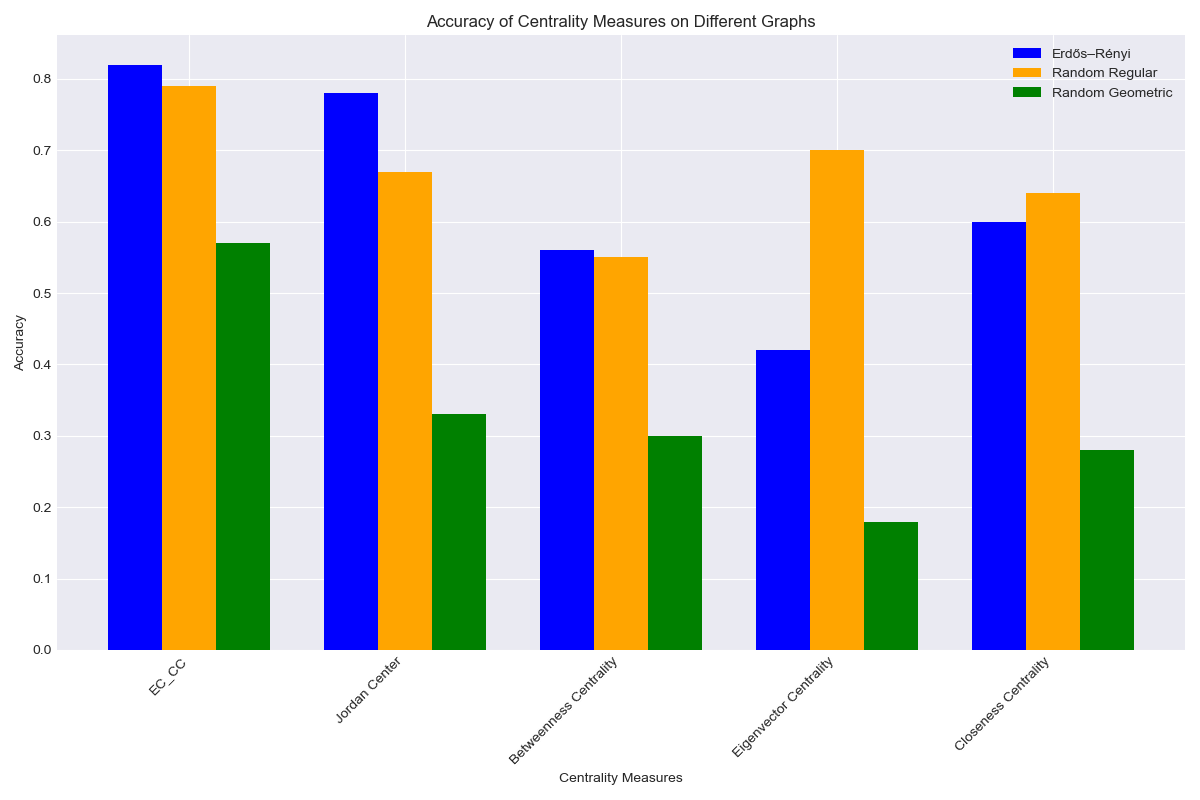
\includegraphics[width=0.8\textwidth]{Accuracy_Centrality_Measures.png}
    \caption{Accuracy of Centrality Measures on Different Graphs}
    \label{fig:accuracy_centrality_measures}
\end{figure}

From the accuracy plot, we observe that the combination of Eccentricity and Closeness Centrality (EC\_CC) consistently demonstrates the highest accuracy across all network types. This is likely because Eccentricity identifies the node that minimizes the maximum distance to all other nodes, while Closeness Centrality ensures that the node is centrally located in terms of average shortest path distances. Together, they provide a robust indication of the central node, which is often the source of the infection.\\

For Erdős–Rényi and Random Regular graphs, the accuracy is relatively high. This can be attributed to the regularity and homogeneity of these graphs, where nodes tend to have similar numbers of neighbors, allowing centrality measures to perform effectively. The consistent connectivity patterns in these graphs make it easier for the algorithms to identify the central nodes accurately.

In contrast, the accuracy is lower for Random Geometric graphs. These graphs have irregular structures, with varying node degrees and connectivity patterns, especially near the boundaries. The irregularities and the presence of boundary nodes, which have fewer neighbors, make it challenging for centrality measures to accurately identify the infection source. The varying density and proximity-based connections disrupt the uniformity, leading to lower accuracy in source detection.\\

However, accuracy is not the only criterion to consider. The computational efficiency of these algorithms is equally important, especially for large-scale networks. Figure \ref{fig:average_time_centrality_measures} illustrates the average time taken by various centrality measures on different network types.

\begin{figure}[H]
    \centering
    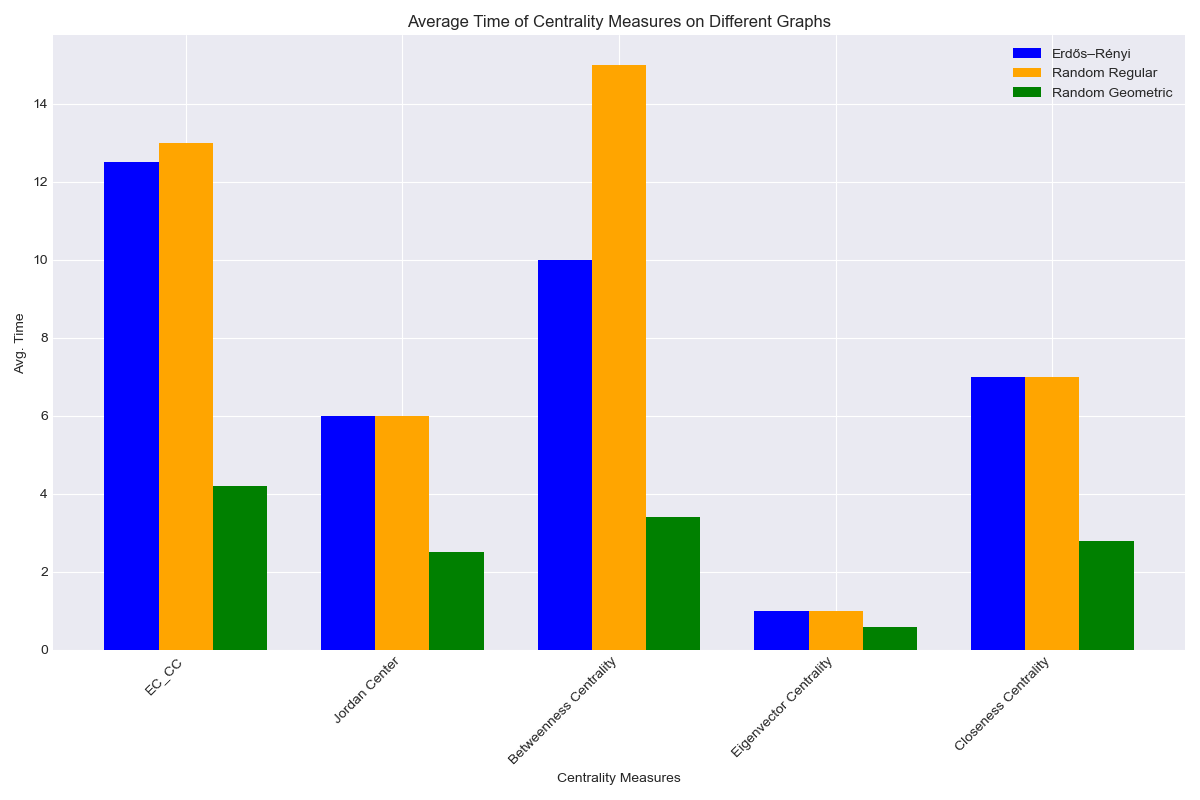
\includegraphics[width=0.8\textwidth]{Average_Time_Centrality_Measures.png}
    \caption{Average Time of Centrality Measures on Different Graphs}
    \label{fig:average_time_centrality_measures}
\end{figure}

The combination of Eccentricity and Closeness Centrality (EC\_CC), while accurate, is the most time-consuming. This is because these measures involve complex calculations that consider the distances between all pairs of nodes. The high time complexity can be a significant drawback in large networks where quick decision-making is crucial.

Betweenness Centrality also takes a considerable amount of time due to its dependency on the shortest paths between all node pairs. It provides valuable insights into the network's flow structure but at the cost of computational efficiency.

Eigenvector Centrality is relatively fast but sacrifices accuracy, particularly in irregular networks. It assigns scores based on the principle that connections to high-scoring nodes contribute more to a node's score. While this is useful in some contexts, it may not always accurately identify the infection source, especially in heterogeneous networks.

Closeness Centrality strikes a balance between time and accuracy, performing well across different network types. It measures the average length of the shortest path from a node to all other nodes, providing a good indication of centrality without the computational overhead of Betweenness or EC\_CC.

Jordan Centrality provides a favorable balance between accuracy and time complexity, making it an excellent choice for source detection algorithms. It performs effectively on both grid-based and network-based models.\\

In summary, the choice of centrality measure depends on the specific requirements of the analysis. For high accuracy, especially in regular networks, EC\_CC is preferred despite its higher computational cost. For faster computations, Eigenvector or Closeness Centrality might be more suitable, particularly in large or irregular networks.\\

The results from our study highlight the strengths and weaknesses of various centrality measures for source detection in complex networks. By understanding these trade-offs, we can select the most appropriate algorithm based on the network structure and the specific requirements of the task at hand.

\section{Stochastic Approach and Comparative Analysis}

Incorporating stochastic elements into the infection spread models captures the randomness observed in real-world scenarios \cite{liu2020}. We used Stochastic Differential Equations (SDEs) to model these random fluctuations. The SDEs for the SIRS model incorporate Wiener processes to account for random perturbations in the state of susceptible, infected, and recovered individuals, as presented in equations \ref{equation:3.4}, \ref{equation:3.5}, and \ref{equation:3.6} in the background chapter \cite{paladini2011}.\\

To simulate these stochastic models, we employed the Gillespie Algorithm, which is particularly suitable for simulating the time evolution of systems with random events, such as the spread of infectious diseases. The flowchart of the Gillespie Algorithm is shown in Figure \ref{fig:gillespie_algorithm}.

\begin{figure}[H]
    \centering
    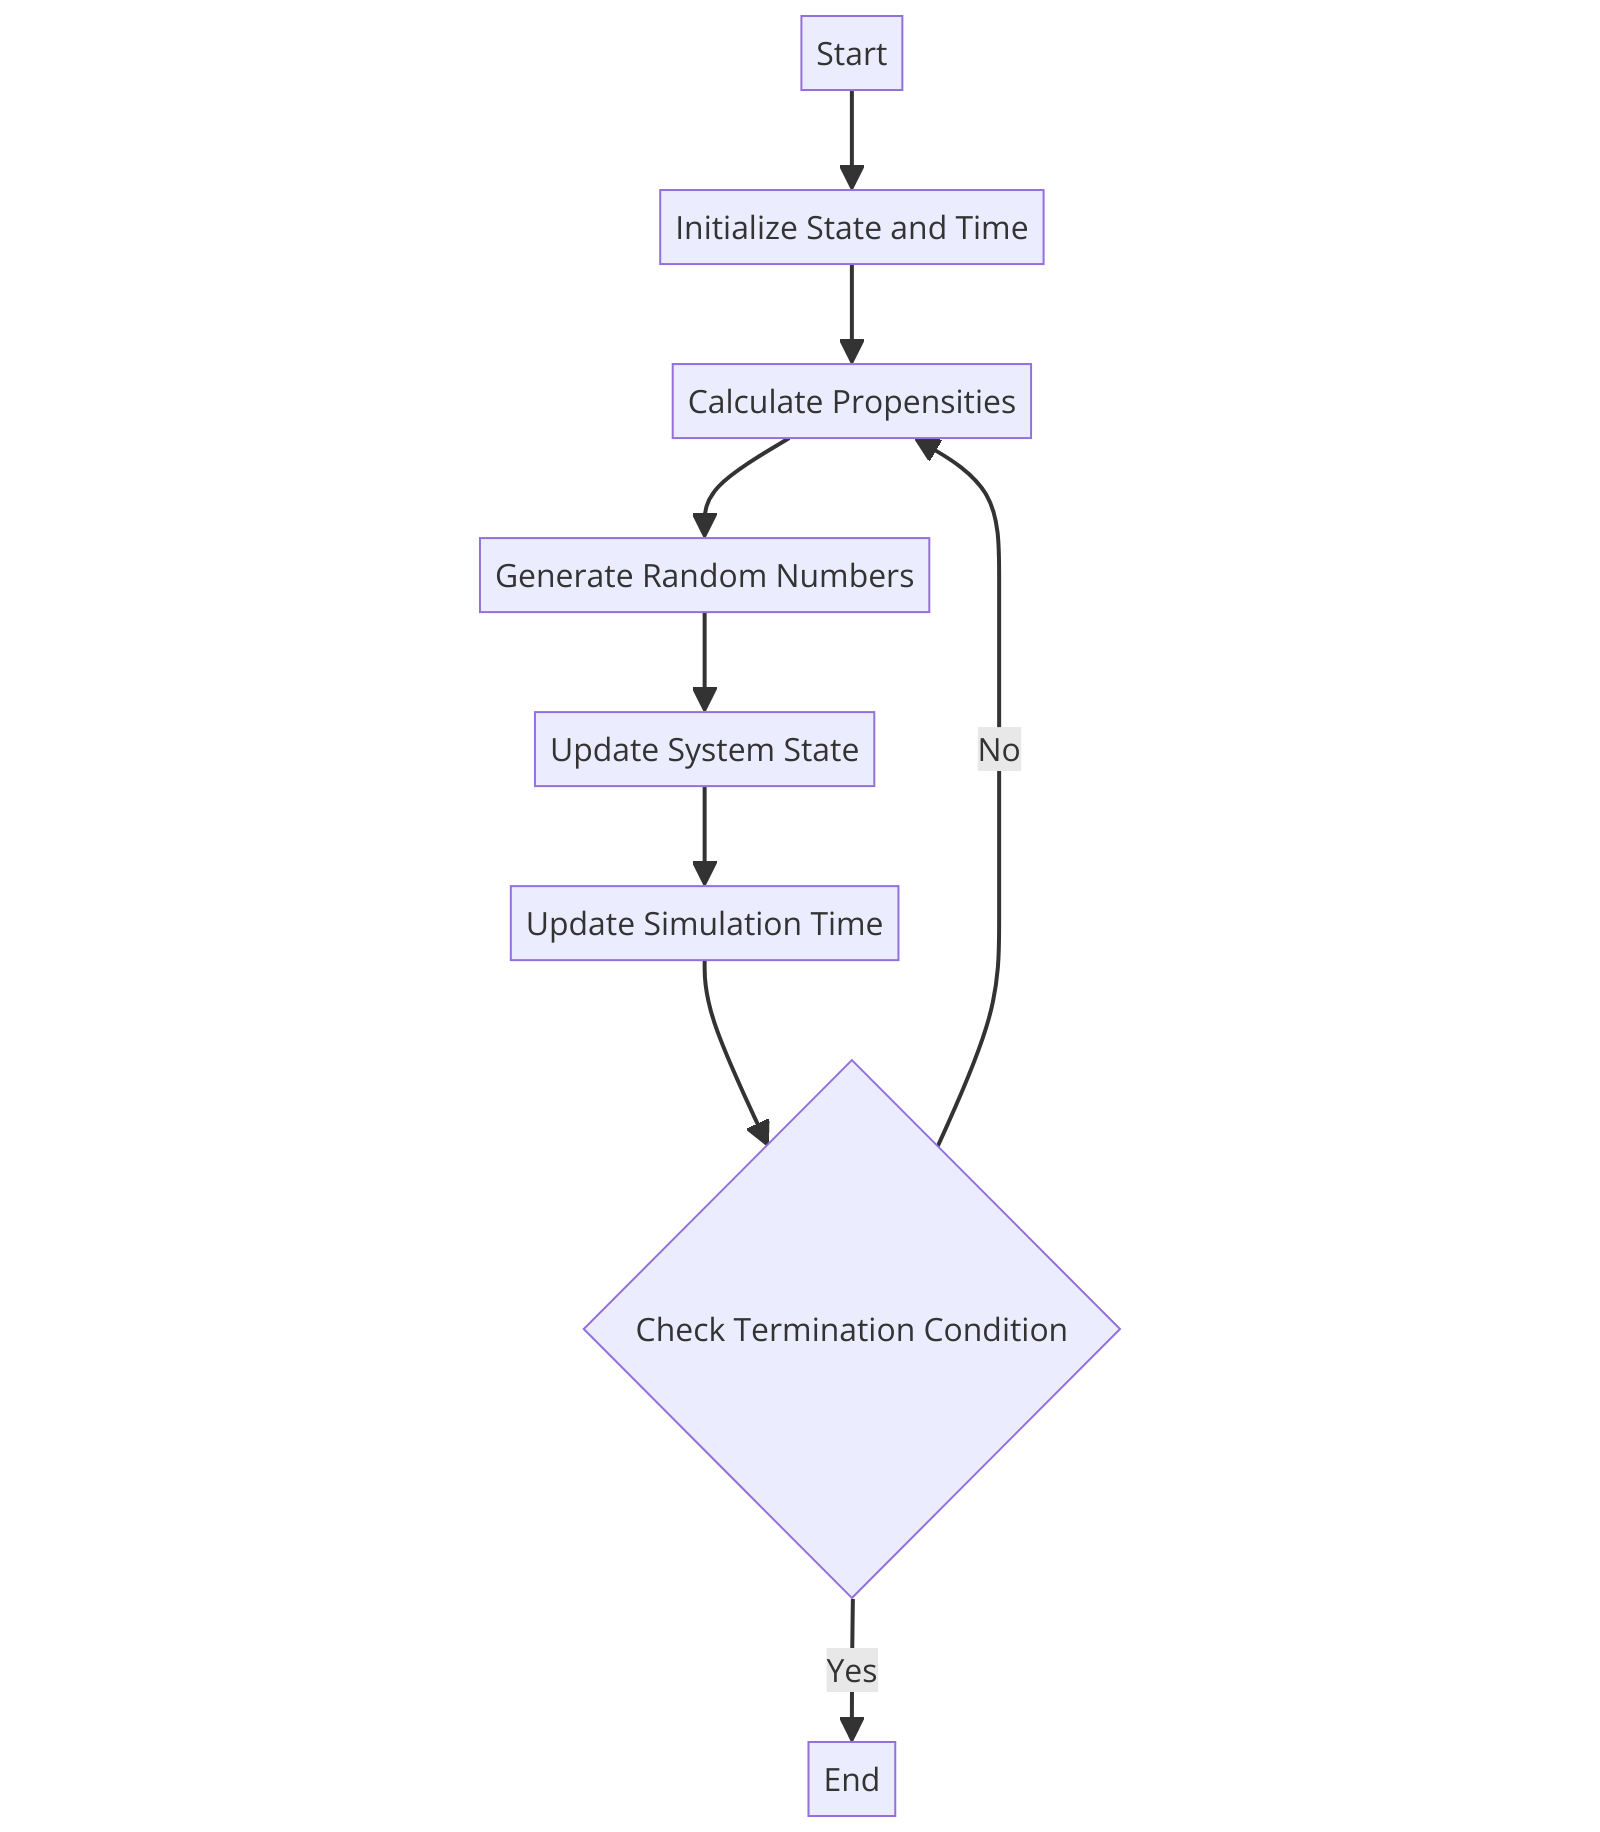
\includegraphics[width=0.8\textwidth]{flowchart_algorithm.png}
    \caption{Flowchart of the Gillespie Algorithm}
    \label{fig:gillespie_algorithm}
\end{figure}

The Gillespie Algorithm allows us to model the discrete nature of infection events and the inherent randomness in the timing of these events. By incorporating stochastic elements, we can capture the unpredictable fluctuations that occur in real-world disease spread scenarios. The algorithm randomly determines the time to the next event and which event will occur, ensuring that the inherent randomness in infection and recovery processes is accurately represented.

To highlight the impact of randomness on disease spread and source detection, we performed a comparative analysis between the stochastic and deterministic approaches. The comparison revealed that stochastic models provide a more realistic simulation of infection dynamics, accounting for the inherent uncertainties in real-world scenarios. The comparison of stochastic and deterministic models is illustrated in Figure \ref{fig:stochastic_vs_deterministic}. The detailed steps of the algorithm are explained in the Implementation chapter.

\begin{figure}[H]
    \centering
    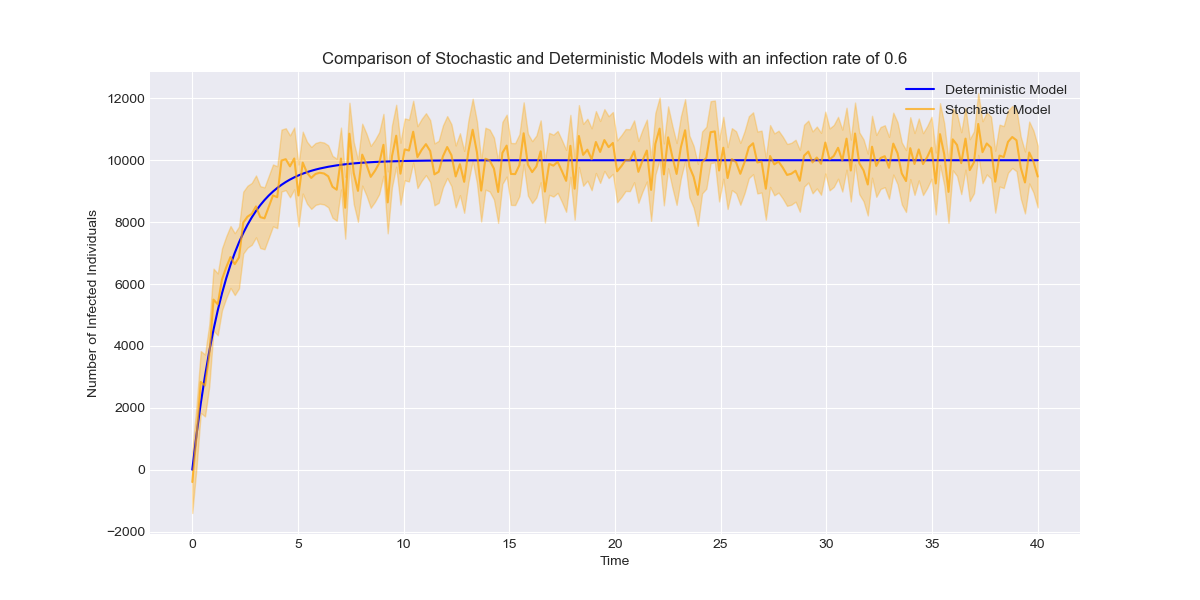
\includegraphics[width=0.8\textwidth]{stochastic_vs_deterministic.png}
    \caption{Comparison of Stochastic and Deterministic Models}
    \label{fig:stochastic_vs_deterministic}
\end{figure}

From Figure \ref{fig:stochastic_vs_deterministic}, we can observe that the stochastic model captures the variability and noise present in real-world data, leading to more robust and reliable predictions of disease spread and source detection. In contrast, the deterministic model, while useful for understanding baseline behavior, often fails to capture the variability and unpredictability seen in real-world scenarios. This highlights the importance of incorporating stochastic elements into epidemiological models.\\

The stochastic approach, modeled using the Gillespie Algorithm, offers several advantages:

\begin{itemize}
    \item It captures the randomness and variability observed in real-world infection spread, which deterministic models may overlook.
    \item It provides a more nuanced understanding of disease dynamics by accounting for random fluctuations and noise.
    \item It leads to more robust and reliable predictions of disease spread and source detection, as it better reflects the inherent uncertainties in real-world scenarios.
\end{itemize}

In deterministic models, the infection spread follows a predictable path based on initial conditions and fixed parameters, leading to a single, smooth trajectory. However, real-world epidemics are influenced by numerous unpredictable factors, such as individual behavior variations, environmental changes, and random events affecting transmission. Stochastic models, by incorporating random noise and fluctuations, provide a range of possible outcomes, reflecting the true nature of disease spread.

For instance, in stochastic models, the equilibrium state of the disease dynamics may vary between simulations, capturing the inherent uncertainty in real-world scenarios. This variability can affect the performance of source detection algorithms, as the spread patterns are less predictable and more diverse. The deterministic models, while useful for a baseline understanding, may miss these variations, leading to less accurate predictions in practical applications.\\

In summary, incorporating stochastic elements into infection spread models significantly enhances their realism and reliability. The stochastic models account for the inherent randomness and noise present in real-world disease spread, leading to more accurate and robust predictions. This comparative analysis underscores the importance of stochastic modeling in epidemiological research and the need for further development of these models to better understand and control disease spread.

\section{Conclusion}

This chapter has detailed the design and implementation of grid-based and complex network models for simulating infectious disease spread. By employing various source detection algorithms and centrality measures, we aimed to improve the traceability of infection sources. The integration of stochastic elements further enhanced the realism of our simulations, providing a comprehensive framework for understanding disease dynamics.

The Jordan Center algorithm demonstrated high accuracy in wrap-around grid configurations but showed limitations in fixed boundary scenarios. Centrality measures like EC\_CC proved to be the most effective for source detection in complex networks, although at the cost of higher computational time.\\

In summary, our findings highlight the importance of selecting appropriate algorithms and centrality measures based on the network structure and the specific requirements of the analysis. The choice of algorithm significantly impacts the accuracy and computational efficiency of source detection in epidemiological models.